\chapter{Methodology}
We have implemeted a quantitative approach for the study of Cross-Dataset Generalization for Network Intrusion Detection Using Supervised and Unsupervised Machine Learning Models. 
The study focuses on the overall performance of the models in detection of 'Attack' from the test datasets by training the models on an entire train dataset. Since the focus of this 
study is to investigate the cross-dataset generalization capabilities of both supervised and unsupervised machine learning models for network intrusion detection, the models will be 
trained entirely on CIC-IDS-2017 dataset and evaluated on unseen CSE-CIC-IDS2018 and UNSW-NB15 datasets.

\begin{itemize}[nosep, leftmargin=*, itemsep=0pt, parsep=0pt, topsep=2pt]
    \item \textbf{Research Type:} Quantitative
    \item \textbf{Data:} Publicly available datasets
        \begin{itemize}
            \item \textbf{Train Dataset:} CIC-IDS-2017
            \item \textbf{Test Dataset:} CSE-CIC-IDS2018 and UNSW-NB15
            \end{itemize}
    \item \textbf{Sampling:} Non-Random Sampling
            \begin{itemize}
                \item Convenience Sampling
            \end{itemize}   
    \item \textbf{Programming Language:} Python 3.11
    \item \textbf{Libraries:} Pandas, Numpy, Tensorflow, Keras, Scikit-learn, Optuna, RobustScaler, Matplotlib, Seaborn
    \item \textbf{Models:} Random Forest, XGBoost, DNN, Isolation Forest, One-Class SVM, Autoencoder
    \item \textbf{Evaluation Metrics:} F1-Score, MCC, ROC-AUC Curve
\end{itemize}

\begin{figure}[H]
\centering
\resizebox{0.72\textwidth}{!}{%
\begin{tikzpicture}[
  mainbox/.style={rectangle, rounded corners, draw=mygreen, very thick,
                  fill=white, minimum width=4.4cm, minimum height=1.3cm,
                  align=center, font=\small},
  annobox/.style={rectangle, rounded corners, draw=mygreen, very thick,
                  fill=white, align=center, font=\small,
                  text width=6.2cm, inner sep=8pt},
  myarrow/.style={-{Latex[length=2.8mm]}, mygreen, thick},
  myline/.style={mygreen, thick}
]

% ===== Main pipeline (left column) =====
\node[mainbox] (collect)    at (0,0)      {Data Collection and Loading};
\node[mainbox] (preprocess) at (0,-2.2)   {Data Pre-Processing};
\node[mainbox] (feature)    at (0,-4.4)   {Feature Engineering};
\node[mainbox] (train)      at (0,-6.6)   {Model Training};
\node[mainbox] (eval)       at (0,-8.8)   {Model Evaluation};
\node[mainbox] (deploy)     at (0,-11.0)  {Model Selection and Deployment};

\draw[myarrow] (collect)    -- (preprocess);
\draw[myarrow] (preprocess) -- (feature);
\draw[myarrow] (feature)    -- (train);
\draw[myarrow] (train)      -- (eval);
\draw[myarrow] (eval)       -- (deploy);

% ===== Right-side annotation: data loading =====
\node[annobox] (loadchunk) at (10,0)
  {Load in chunks with memory optimization to avoid memory crash};
\draw[myarrow] (collect.east) -- (loadchunk.west);

% ===== Right-side annotation group 1: Data Pre-Processing's 3 steps =====
\node[annobox] (map_labels)    at (10,-1.6)
  {Mapping the labels (standardizing the labels for all the datasets)};
\node[annobox] (handle_nan)    at (10,-4.4)
  {Handle infinities, NaNs and Duplicates};
\node[annobox] (common_labels) at (10,-7.2)
  {Take only the common labels from the datasets. Remove bad rows if any.};

\draw[decorate, decoration={brace, amplitude=6pt, mirror}, mygreen, thick]
  (6.3,-1.6) -- (6.3,-7.2);

\draw[myline] (6.3,-1.6) -- (map_labels.west);
\draw[myline] (6.3,-4.4) -- (handle_nan.west);
\draw[myline] (6.3,-7.2) -- (common_labels.west);

% Arrow from Data Pre-Processing box to its own brace group
\draw[myarrow] (preprocess.east) -- (6.3,-4.4);

% ===== Right-side annotation group 2: Feature Engineering's 2 subsections =====
\node[annobox] (mapattacks)   at (10,-9.6)
  {Map Attacks};
\node[annobox] (robustscaler) at (10,-11.8)
  {RobustScaler for DNN to handle class imbalance};

\draw[decorate, decoration={brace, amplitude=6pt, mirror}, mygreen, thick]
  (6.3,-9.6) -- (6.3,-11.8);

\draw[myline] (6.3,-9.6)  -- (mapattacks.west);
\draw[myline] (6.3,-11.8) -- (robustscaler.west);

% Arrow from Feature Engineering box to its own brace group
\draw[myarrow] (feature.east) -- (6.3,-10.7);

\end{tikzpicture}%
}
\caption{Workflow for Cross-Dataset Generalization for Network Intrusion Detection.}
\label{fig:methodology-pipeline}
\end{figure}

\section{Dataset Collection and Loading}

For the study of Cross-Dataset Generalization for Network Intrusion Detection Using Supervised and Unsupervised Machine Learning Models at an academic level, 
we have sourced three datasets from public domain. The collected data are then loaded in chunks with memory optization (dowcasting some datatypes) to avoid memory crash.
\begin{table}[htbp]
    \centering
    \caption{Dataset Details}
    \label{tab:dataset-details}

    {\fontsize{9}{11}\selectfont
    \renewcommand{\arraystretch}{1.25}

    \begin{tabularx}{\textwidth}{
        >{\raggedright\arraybackslash}p{2.0cm}
        >{\raggedright\arraybackslash}p{2.4cm}
        >{\raggedright\arraybackslash}X
        >{\centering\arraybackslash}p{1.8cm}
        >{\centering\arraybackslash}p{2.0cm}
        >{\centering\arraybackslash}p{1.8cm}
    }

        \toprule

        \textbf{Dataset} &
        \textbf{Source} &
        \textbf{Link for the Source} &
        \textbf{Dataset Size} &
        \textbf{Dataset Shape} &
        \textbf{Access Date} \\

        \midrule

        CIC-IDS-2017 &
        Kaggle &
        \url{https://www.kaggle.com/datasets/chethuhn/network-intrusion-dataset} &
        884.65 MB &
        2,830,743, 79 &
        22/06/2026 \\

        CSE-CIC-IDS2018 &
        Kaggle &
        \url{https://www.kaggle.com/datasets/solarmainframe/ids-intrusion-csv} &
        6.89 GB &
        16,233,002, 84 &
        22/06/2026 \\

        UNSW-NB15 &
        Canadian Institute for Cybersecurity &
        \url{https://cicresearch.ca/CICDataset/CIC-UNSW/} &
        1.78 GB &
        3,540,241, 84 &
        22/06/2026 \\

        \bottomrule

    \end{tabularx}
    }
\end{table}

CIC-IDS-2017 and CSE- CIC-IDS2018 datasets were downloaded from Kaggle. Meanwhile, the UNSW-NB15 dataset was fetched from Canadian Institute for 
Cybersecurity portal by submitting necessary information. We will employ CIC-IDS-2017 as the train dataset, while CSE- CIC-IDS2018 and UNSW-NB15 
will be our test datasets for cross-dataset generalization for NIDS. A quick exploration of these datasets before data pre-processing showed dominant 
presence of ‘Benign’ class in all the datasets. 2273097 (80.3\%) in CIC-IDS-2017, 13484708 (83.06\%) in CSE- CIC-IDS2018 and 3450658 (97.46\%) in UNSW-NB15 
are labeled as ‘Benign’ indicating huge class imbalance between the benign and attack classes.

\subsection{CIC-IDS-2017}
The dataset consists of network traffics collected from Monday to Friday at different time intervals originally extracted by the Canadian 
Institute for Cybersecurity for the study of network intrusion detection. CIC-IDS-2017 datasets were generated utilizing CICFlowMeter to 
create network flows and labelled them according to timestamps, source and target IP address, source and target ports, communication protocol 
and attack types. To prepare a realistic background traffic, Canadian Institute for Cybersecurity (CIC) applied the suggested B-Profile system \cite{Sharafaldin2018} 
to model the abstract patterns of human interactions and generate the realistic benign background traffic from 25 real users. 
The 8 files combined has 79 features and 2830743 rows.

\subsection{CSE-CIC-IDS2018}
Among all the datasets used for our research, this one is the biggest in size (10 files of 6.89 GB) with more than 16 million rows and 
84 feature downloaded through Kaggle. CSE- CIC-IDS2018 was a collaborative initiative between CIC and Communications Security Establishment 
(CSE) with the objective of creating standard benchmark datasets for intrusion detection systems to properly detect network anomalies. 
The dataset was generated based on different attack types such as Botnets, Brute force, DoS and Heartbleed by accessing different user 
profiles. The dataset is comprised of 80 features obtained through incoming network traffic and system logs with CICFlowMeter-V3 tool with 
proper utilization of B-profile and M-profile to identify the statistical user behavior through the reproduction of network traffics and 
attack scenarios. The initiative used Slowloris and LOIC to inject HTTP DoS attacks, HOIC for DDoS, and bombarded web applications with 
Damn Vulnerability Web App (DVWA) to test the vulnerabilities.


\subsection{UNSW-NB15}

CIC-UNSW-NB15 or simply UNSW-NB15 augmented dataset was created with the help of IXIA PerfectStorm with up-to-date normal and abnormal 
network traffic. The dataset contains 9 types of attacks which the CIC-IDS-2017 and CSE- CIC-IDS2018 datasets lack. CICFlowmeter extracted 
new features from the network flow. The attacks in UNSW-NB15 are categorized by matching the flow records: source/destination IP, port, and 
protocols with the records from ground truth file. UNSW-NB15 prioritized matching Timestamp in-case of multiple records, removed flows that 
could not be categorized and categorized the remaining traffic as benign after malicious flows were processed. 

\section{Data Pre-Processing}
The first step in data-processing is standardizing all the labels across the datasets. We mapped the labels of the datasets taking reference to 
CSE-CIC-IDS2018. We handled the infinite values in these datasets by replacing them with NaN values. Removing duplicates earlier would significantly 
reduce the size of the datasets, seeing the skewness of the datasets, we replaced the NaN values with the median values from the respective labels. 
And, only after replacing the NaN values with median values, we removed the duplicated values from the datasets. Finally, for the next step we took 
all the common labels from the datasets. We also checked and deleted the bad rows from the datasests.

\section{Feature Engineering}
In order to maximize the intrusion detection, we mapped the attacks of similar nature. Since, the tree based models are robust in handling the class-imbalance, 
we have simply implemented class-weighting and avoided using SMOTE for Random Forest and XGBoost. Meanwhile, for our DNN architecture, we used RobustScaler to 
fit-transform the train datasets only.

\section{Model Training}
\subsection{Random Forest}
Random Forest is a robust ensemble learning model that creates many decision trees and carries out classification by taking the mode of the 
predictions of individual trees. During the training phase, only a random subset of features is considered at each node split. The trees in 
a random forest use a bootstrap-sampled version of the training data to introduce randomness in both the sampling process and feature selection, 
thereby minimizing correlation among the trees and reducing the variance of the ensemble without increasing bias.

\begin{wrapfigure}{l}{0.65\textwidth}
    \centering
    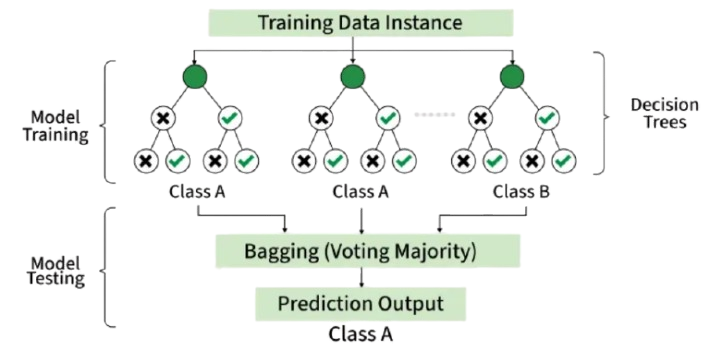
\includegraphics[
        width=0.60\textwidth,
        height=7cm,
        keepaspectratio
    ]{attachments/random forest.png}
    \caption{Random Forest Architecture}
    \label{fig:random-forest}
\end{wrapfigure}

The significance of tree-based models lies in their ability to classify the feature space using threshold splits without being affected by 
monotonic transformations of the input features. In this study, we trained Random Forest on the full CIC-IDS-2017 dataset without scaling, 
despite the substantial class imbalance. As Random Forest is resistant to overfitting on high-dimensional flow-related data and shows robustness 
to noisy features, the workflow avoids Synthetic Minority Over-Sampling Technique (SMOTE) and instead uses class weight = "balanced" to 
handle class imbalance. \par
\clearpage

\begin{table}[!ht]
    \centering
    \caption{Hyperparameters for Random Forest}  
    \label{tab:Hyperparameters-details Random Forest}
    {\fontsize{9}{11}\selectfont
    \renewcommand{\arraystretch}{1.25}
    \begin{tabularx}{\textwidth}{
        >{\raggedright\arraybackslash}p{3.5cm}
        >{\centering\arraybackslash}p{2.0cm}
        >{\raggedright\arraybackslash}X
    }

        \toprule

        \textbf{Hyperparameter} &
        \textbf{Value} &
        \textbf{Purpose} \\

        \midrule

        n\_estimators &
        200 &
        Number of trees in the forest \\

        max\_depth &
        10 &
        Maximum depth of each tree \\

        min\_samples\_split &
        2 &
        Minimum samples to split an internal node \\

        min\_samples\_leaf &
        2 &
        Minimum samples for each leaf node \\

        max\_features &
        sqrt &
        Number of features at each split \\

        bootstrap &
        True &
        Bootstrap sampling to build trees \\

        
        criterion &
        gini &
        Function to measure split quality \\

        class\_weight &
        balanced &
        To automatically address the class imbalance \\

        random\_state &
        42 &
        Seed for reproducibility \\

        n\_jobs &
        -1 &
        Parallel Processing \\

        \bottomrule
    \end{tabularx}
    }
\end{table}
\FloatBarrier

\subsection{XGBoost}
eXtreme Gradient Boosting generally termed as XGBoost is a scalable gradient boosting decision tree which boost weak learners. XGBoost utilizes the technique 
where each tree is trained to rectify the mistakes of previous trees. It does not build trees based on parallel bagging as Random Forest does. Rather XGBoost 
allows trees to grow in additive way to optimize the differential loss function using gradient descent. It employs L1 and L2 regularization to control overfitting 
and complexity. XGBoost inhibits computational effectiveness and robustness in solving structured data and is capable to construct parallel tree to deal with the 
missing data.
\begin{wrapfigure}{l}{0.60\textwidth}
    \centering
    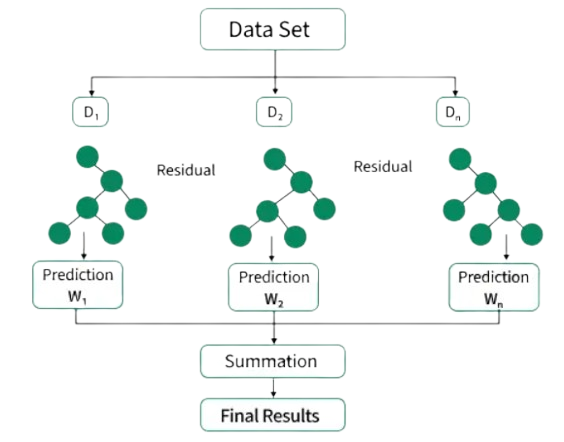
\includegraphics[
        width=0.85\textwidth,
        height=7cm,
        keepaspectratio
    ]{attachments/xgboost.png}
    \caption{XGBoost Architecture}
    \label{fig:xgboost}
\end{wrapfigure}

So, with its exceptional ensemble technique to compare methods of ensemble trees that differ in aggregation approach (sequential vs parallel), 
we have selected XGBoost along with Random Forest as our benchmark supervised learning models. Like random forest, we have implemented 
class-weighing to mitigate the class imbalance between the benign and malicious cases in the training set, i.e. CIC-IDS-2017. 
\par
\clearpage

\begin{table}[!ht]
    \centering
    \caption{Hyperparameters for XGBoost}  
    \label{tab:Hyperparameters-details XGBoost}
    {\fontsize{9}{11}\selectfont
    \renewcommand{\arraystretch}{1.25}
    \begin{tabularx}{\textwidth}{
        >{\raggedright\arraybackslash}p{3.5cm}
        >{\centering\arraybackslash}p{2.0cm}
        >{\raggedright\arraybackslash}X
    }

        \toprule

        \textbf{Hyperparameter} &
        \textbf{Value} &
        \textbf{Purpose} \\

        \midrule

        n\_estimators &
        200 &
        Number of boosting trees in the forest \\

        max\_depth &
        6 &
        Maximum depth of each tree \\

        learning\_rate &
        0.1 &
        Contribution of each tree to the final model \\

        sub\_sample &
        0.8 &
        Training sub-samples to boost iteration \\

        col\_sample\_bytree &
        0.8 &
        Fraction of features for each tree \\

        objective &
        binary:logistic &
        Specifies binary classification \\

        eval\_metric &
        logloss &
        Metric to calculate classification error \\

        tree\_method &
        hist &
        Histogram based training\\
        
        scale\_pos\_weight &
        neg/pos &
        Handles class imbalance \\

        random\_state &
        42 &
        Seed for reproducibility \\

        n\_jobs &
        -1 &
        Parallel Processing \\

        \bottomrule
    \end{tabularx}
    }
\end{table}
\FloatBarrier

\subsection{Deep Neural Network (DNN)}
DNN learn feature interactions without manual feature extraction giving it an extra edge over tree-based ensemble techniques. 
DNN is dependent on the size/amount of data, thus shows better performance as the degree of changes in inputs rises. DNN uses 
hidden layers for classification. Each hidden layer utilizes ReLU activation to bring in non-linearity after each hidden layer 
to prevent the vanishing gradient problem of deeper models.

\begin{wrapfigure}{l}{0.70\textwidth}
    \centering
    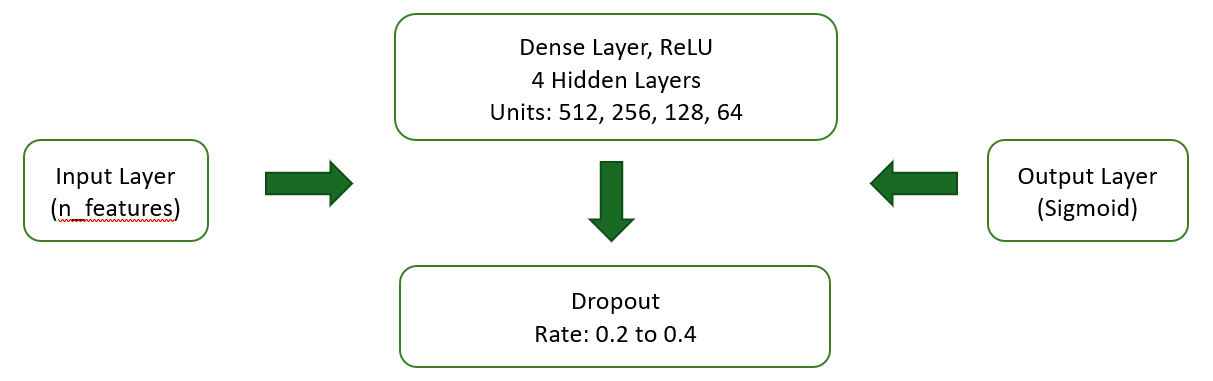
\includegraphics[
        width=0.70\textwidth,
        height=9cm,
        keepaspectratio
    ]{attachments/dnn.png}
    \caption{DNN Architecture for this study}
    \label{fig:dnn}
\end{wrapfigure}

To avoid memory crash given the size of the dataset, we tested on 20\% of the CIC-IDS-2017 with tuning size of 300000. Furthermore, we have 
configured Optuna study which optimizes the hyperprameters of the model \cite{Akiba2019} to get maximum F1 score for the "Attack' class with n\_trials=30 
(30 only considering the computational cost and to prevent memory crash). We have implemented 4 hidden layers with 512, 256, 128 and 64 neurons for binary 
classification “benign” and “attack”  in this study. We have implemented RobustScaler for scaling the datasets to mitigate the effect of strong outliers 
(flow duration, packet inter-arrival times). Similar to Random Forest and XGBoost which utilizes class-weight, weighted loss in DNN handles class imbalance. 
In consideration to the huge test dataset size, prediction and evaluation of the model has been performed in batches of max 4096. The best\_dnn\_params 
identifies the best configuration of the model specifically the number of layers, units per layer, dropout rate and the learning rate to construct the best 
DNN architecture. Thus, the evaluation using DNN architecture works in two phases, first finding the best configuration by training and testing the model 
on CIC-IDS-2017 and secondly using the best hyperparameters to evaluate the performance of the model on the test datasets CSE-CIC-IDS2018 and UNSW-NB15. 
\clearpage

\begin{table}[!ht]
    \centering
    \caption{Hyperparameters for DNN}  
    \label{tab:Hyperparameters-details DNN}
    {\fontsize{9}{11}\selectfont
    \renewcommand{\arraystretch}{1.25}
    \begin{tabularx}{\textwidth}{
        >{\raggedright\arraybackslash}p{3.5cm}
        >{\centering\arraybackslash}p{2.0cm}
        >{\raggedright\arraybackslash}X
    }

        \toprule

        \textbf{Hyperparameter} &
        \textbf{Search Space} &
        \textbf{Purpose} \\

        \midrule

        n\_layers &
        2, 4 &
        Controls network depth, learns complex features and balances overfitting\\

        units per layer&
        [512, 256, 128, 64] &
        Controls width of hidden layer and checks the respresentational capacity at each layer \\

        learning\_rate &
        [1e-4, 1e-2] &
        Controls the step size during gradient descent \\

        dropout\_rate &
        0.1, 0.5 &
        Deactivate the neurons during training to prevent overfitting and overall regularizes the network \\
        
        batch\_size &
        [512, 1024, 2048, 4096] &
        Prevents memory crashes, training speed and gradient noise by controlling the number of samples processed \\

        \bottomrule
    \end{tabularx}
    }
\end{table}
\FloatBarrier
